% Same observed sample, one fixed learner, and two indistinguishable label tables.
% Volume three architecture figures. Independent export only; not book fonts.
\colorlet{MutedBlueFill}{FigureBlueFill}
\colorlet{MutedGreenFill}{FigureGreenFill}
\colorlet{MutedPurple}{FigurePurple}
\colorlet{MutedPurpleFill}{FigurePurpleFill}
\tikzset{
 v3 picture/.style={x=1mm,y=1mm,font=\figurefont\fontsize{8}{10}\selectfont,text=FigureInk,line width=.65pt},
 v3 box/.style={draw=FigureBlue,fill=white,rounded corners=1.35mm,line width=.85pt,inner sep=2.5pt,align=center},
 v3 data/.style={v3 box,fill=FigureBlueFill},
 v3 model/.style={v3 box,draw=FigureGreen,fill=FigureGreenFill},
 v3 output/.style={v3 box,draw=FigureYellow,fill=FigureYellowFill},
 v3 risk/.style={v3 box,draw=FigureRed,fill=FigureRedFill},
 v3 group/.style={draw=FigureBlue,rounded corners=1.7mm,line width=.85pt,inner sep=3mm},
 v3 flow/.style={draw=FigureStroke,line width=.85pt,-{Stealth[length=1.9mm,width=1.25mm]},rounded corners=1.1mm},
 v3 guide/.style={draw=FigureMuted,line width=.6pt,dashed},
 v3 feedback/.style={v3 flow,draw=FigureGreen,dashed},
 v3 title/.style={draw=none,fill=none,font=\figurefont\fontsize{8}{10}\selectfont,align=center,inner sep=1pt},
 v3 note/.style={draw=none,fill=none,font=\FigureNoteFont\fontsize{7.5}{9.5}\selectfont,text=FigureMuted,align=center,inner sep=1pt},
 v3 label/.style={draw=none,fill=none,font=\figurefont\fontsize{8}{10}\selectfont,align=center,inner sep=1pt},
 v3 wire/.style={draw=FigureMuted,line width=.45pt},
 v3 point/.style={circle,draw=FigureBlue,fill=FigureBlueFill,minimum size=2.3mm,inner sep=0pt,line width=.55pt}
}
% Bring pre-existing native TikZ geometry to the same typography and scale.
\tikzset{
 foundation picture/.append style={font=\figurefont\fontsize{8}{10}\selectfont,line width=.65pt},
 foundation node/.append style={rounded corners=1.8pt,line width=.7pt,font=\figurefont\fontsize{8}{10}\selectfont},
 foundation heading/.append style={draw=none,fill=none,font=\figurefont\fontsize{8}{10}\selectfont},
 foundation note/.append style={draw=none,fill=none,font=\FigureNoteFont\fontsize{7.5}{9.5}\selectfont},
 foundation flow/.append style={line width=.75pt,-{Stealth[length=1.65mm,width=1.05mm]}},
 foundation frame/.append style={rounded corners=1.8pt,line width=.7pt},
 foundation edge label/.append style={draw=none,fill=none,font=\figurefont\fontsize{8}{10}\selectfont}
}
% Official Lucide outline icons, consistently used across diagrams. Size in mm.
\newcommand{\VIcon}[5]{\node[inner sep=0pt] at (#2,#3) {\includegraphics[width=#4mm]{figures/06-foundations/00-shared/tikz/icons/#1-#5.pdf}};}
% A neutral network glyph (not a claim about an actual model architecture).
% Coordinates denote its centre; scale 1 gives 13 x 8 mm.
\newcommand{\VNet}[4]{\begin{scope}[shift={(#1,#2)},scale=#3]
 \foreach \a in {-3,0,3}{\foreach \b in {-3,0,3}{\draw[v3 wire] (-5,\a)--(0,\b);}}
 \foreach \a in {-3,0,3}{\draw[v3 wire] (0,\a)--(5,0);}
 \foreach \a in {-3,0,3}{\draw[draw=#4,fill=#4,line width=.55pt] (-5,\a) circle(.9);\draw[draw=#4,fill=white,line width=.55pt] (0,\a) circle(.9);}
 \draw[draw=#4,fill=#4,line width=.55pt] (5,0) circle(.9);
\end{scope}}
\newcommand{\VDots}[4]{\foreach \k in {0,1,2,3}{\fill[#4] ({#1+2.7*\k},#2) circle(#3);}}
% Feature vector/tensor elements are scientific glyphs, not decorative icons.
\newcommand{\VVector}[4]{\foreach \k in {0,...,4}{\fill[#4,rounded corners=.25pt] ({#1+2.2*\k},#2) rectangle ++(1.5,#3);}}
% Detailed glyphs retain the visual vocabulary of the reference drawings.
% Layer counts are explicit: never substitute one topology for every network.
\colorlet{VNetworkInput}{FigureGreen}
\colorlet{VNetworkHidden}{FigureBlue}
\colorlet{VNetworkOutput}{FigureYellow}
\newcommand{\VLayerNetSpacing}[7]{\begin{scope}[shift={(#1,#2)},scale=#3]
 \foreach \i in {1,...,#4}{\foreach \j in {1,...,#5}{
  \draw[FigureStroke!85,line width=.68pt] (-7,{(\i-(#4+1)/2)*#7})--(0,{(\j-(#5+1)/2)*#7});}}
 \foreach \i in {1,...,#5}{\foreach \j in {1,...,#6}{
  \draw[FigureStroke!85,line width=.68pt] (0,{(\i-(#5+1)/2)*#7})--(7,{(\j-(#6+1)/2)*#7});}}
 \foreach \i in {1,...,#4}{\draw[draw=FigureStroke!85,fill=VNetworkInput!60!white,line width=.8pt] (-7,{(\i-(#4+1)/2)*#7}) circle(1.15);}
 \foreach \i in {1,...,#5}{\draw[draw=FigureStroke!85,fill=VNetworkHidden!48!white,line width=.8pt] (0,{(\i-(#5+1)/2)*#7}) circle(1.15);}
 \foreach \i in {1,...,#6}{\draw[draw=FigureStroke!85,fill=VNetworkOutput!70!white,line width=.8pt] (7,{(\i-(#6+1)/2)*#7}) circle(1.15);}
\end{scope}}
\newcommand{\VLayerNet}[6]{\VLayerNetSpacing{#1}{#2}{#3}{#4}{#5}{#6}{3.6}}
\newcommand{\VLayerNetTall}[6]{\VLayerNetSpacing{#1}{#2}{#3}{#4}{#5}{#6}{6.0}}
% Operators follow the DP-SGD visual grammar: a quiet rounded surround,
% a stronger circular core, and one readable mathematical operation.
% Arguments: node name, centre x/y, surround size (mm), semantic colour, math.
\newcommand{\VOperator}[6]{%
 \pgfmathsetmacro{\VOperatorCore}{#4*.74}%
 \node[draw=none,fill=#5!12!white,rounded corners=1.8pt,
   minimum width=#4mm,minimum height=#4mm,inner sep=0pt] (#1-outer) at (#2,#3) {};
 \node[circle,draw=#5,fill=#5!32!white,line width=.9pt,
   minimum size=\VOperatorCore mm,inner sep=.4pt,
   font=\figurefont\fontsize{10.5}{11.5}\selectfont,text=FigureInk] (#1) at (#2,#3) {$#6$};}
% Gaussian noise is a mechanism glyph, with the same surround and circle.
\newcommand{\VNoise}[5]{%
 \VOperator{#1}{#2}{#3}{#4}{#5}{}%
 \begin{scope}[shift={(#2,#3)},scale={#4/12}]
  \path[draw=#5,fill=#5!65!white,line width=.9pt]
    (-3,-1.9)--plot[domain=-3:3,samples=36] (\x,{-1.9+4.2*exp(-\x*\x/2)})--cycle;
 \end{scope}}
% Filled envelopes and folded sheets: thin strokes, distinct internal details.
\newcommand{\VEnvelope}[4]{\begin{scope}[shift={(#1,#2)},scale=#3,line join=round]
 \draw[draw=#4!85!FigureStroke,fill=#4!16!white,line width=.85pt,rounded corners=.7pt] (-6,-4) rectangle (6,4);
 \draw[draw=#4!85!FigureStroke,line width=.8pt] (-5.8,-3.7)--(-1,0.1) (5.8,-3.7)--(1,0.1);
 \draw[draw=#4!85!FigureStroke,fill=white,line width=.85pt] (-5.8,3.8)--(0,-.7)--(5.8,3.8);
\end{scope}}
\newcommand{\VDocument}[4]{\begin{scope}[shift={(#1,#2)},scale=#3,line join=round,line cap=round]
 \draw[draw=#4!85!FigureStroke,fill=#4!13!white,line width=.85pt,rounded corners=.4pt] (-4,-5.2)--(4,-5.2)--(4,2.5)--(1.5,5.2)--(-4,5.2)--cycle;
 \draw[draw=#4!85!FigureStroke,fill=#4!32!white,line width=.8pt] (1.5,5.2)--(1.5,2.5)--(4,2.5);
 \foreach \y/\len in {1.3/2.7,-.6/4.5,-2.5/4.5}{\draw[draw=#4!85!FigureStroke,line width=1pt] (-2.2,\y)--++(\len,0);}
\end{scope}}
\newcommand{\VDatabase}[4]{\begin{scope}[shift={(#1,#2)},scale=#3]
 \draw[draw=#4!85!FigureStroke,fill=#4!30!white,line width=.85pt] (-5.5,-4.5)--(-5.5,4.5) arc(180:360:5.5 and 1.8)--(5.5,-4.5) arc(0:-180:5.5 and 1.8);
 \draw[draw=#4!85!FigureStroke,line width=.8pt] (-5.5,-1.5) arc(180:360:5.5 and 1.8) (-5.5,1.5) arc(180:360:5.5 and 1.8);
 \draw[draw=#4!85!FigureStroke,fill=#4!48!white,line width=.85pt] (0,4.5) ellipse(5.5 and 1.8);
\end{scope}}
\newcommand{\VGear}[4]{\begin{scope}[shift={(#1,#2)},scale=#3]
 \path[fill=#4,rounded corners=.35pt] (-18:3.5)
  \foreach \a in {0,36,...,324}{--({\a-12}:3.5)--({\a-12}:4.4)--({\a+12}:4.4)--({\a+12}:3.5)--({\a+18}:3.5)}--cycle;
 \fill[white] (0,0) circle(1.65);
\end{scope}}
\newcommand{\VGears}[4]{\VGear{#1-2.3}{#2+1.1}{#3}{#4}\VGear{#1+4.2}{#2-3.0}{#3*.55}{#4}}
\newcommand{\VBrowser}[4]{\begin{scope}[shift={(#1,#2)},scale=#3,line cap=round]
 \draw[draw=#4!85!FigureStroke,fill=white,rounded corners=1pt,line width=.7pt] (-10,-7.5) rectangle (10,7.5);
 \path[fill=#4!35!white,rounded corners=1pt] (-9.7,4.6) rectangle (9.7,7.2);
 \draw[draw=#4!85!FigureStroke,line width=.65pt] (-10,4.5)--(10,4.5);
 \foreach \x in {-8.4,-6.8,-5.2}{\fill[#4!85!FigureStroke] (\x,5.9) circle(.4);}
 \fill[#4!12!white] (-9.7,-7.2) rectangle (-3.3,4.2);
 \foreach \y in {2.3,.5,-1.3}{\draw[#4!55!white,line width=1.6pt] (-8,\y)--(-5,\y);}
 \fill[#4!35!white,rounded corners=.5pt] (-1.8,-.2) rectangle (8.4,2.8);
 \fill[FigureGreen!35!white,rounded corners=.5pt] (4.7,-5.4) rectangle (8.4,-1.8);
 \foreach \y in {-2,-3.5,-5}{\draw[#4!40!white,line width=.9pt] (-1.8,\y)--(3.2,\y);}
\end{scope}}
\newcommand{\VRobot}[3]{\begin{scope}[shift={(#1,#2)},scale=#3,line join=round,line cap=round]
 \draw[draw=FigurePurple!85!FigureStroke,fill=FigurePurple!38!white,line width=.7pt] (-6,-7)--(-7,1)--(-1,6)--(4,2)--(2,0)--(-1,3)--(-4,0)--(-3,-7)--cycle;
 \foreach \x/\y/\r in {-5.5/0/1.8,-.7/5/1.65,3.8/1.5/1.25}{
  \draw[draw=FigurePurple!85!FigureStroke,fill=FigurePurple!45!white,line width=.7pt] (\x,\y) circle(\r);
  \fill[white] (\x,\y) circle(.65);}
 \draw[draw=FigureBlue!85!FigureStroke,fill=FigureBlue!35!white,line width=.65pt] (3.1,.4)--(2,-1.2)--(2.8,-2.9)--(3.5,-2.3)--(3,-1.3)--(4.2,-.2)--(5.2,-1.3)--(4.7,-2.3)--(5.4,-2.9)--(6.2,-1.2)--(5,.4);
 \draw[draw=FigurePurple!85!FigureStroke,fill=FigurePurple!38!white,rounded corners=.6pt,line width=.7pt] (-7.8,-8.6)--(-7.8,-7.1) .. controls (-7.8,-6) and (-1.2,-6) .. (-1.2,-7.1)--(-1.2,-8.6)--cycle;
\end{scope}}
\newcommand{\VPerson}[4]{\begin{scope}[shift={(#1,#2)},scale=#3]
 \fill[#4] (0,2.8) circle(1.9);
 \path[fill=#4,rounded corners=.5pt] (-3.3,-3.5)--(-3.3,-1.5) .. controls (-3.3,1.6) and (3.3,1.6) .. (3.3,-1.5)--(3.3,-3.5)--cycle;
\end{scope}}
\newcommand{\VServer}[4]{\begin{scope}[shift={(#1,#2)},scale=#3]
 \foreach \y in {-3,0,3}{
  \draw[draw=#4!85!FigureStroke,fill=#4!75!white,line width=.55pt,rounded corners=.6pt] (-5,\y-1.2) rectangle (5,\y+1.2);
  \fill[white] (3.8,\y) circle(.3);
  \draw[#4!30!white,line width=.55pt] (-3.5,\y)--(-.5,\y);}
\end{scope}}
\newcommand{\VMonitor}[4]{\begin{scope}[shift={(#1,#2)},scale=#3]
 \draw[draw=#4!85!FigureStroke,fill=#4!25!white,line width=.7pt,rounded corners=.6pt] (-6,-3.6) rectangle (6,4.3);
 \fill[white] (-5.2,-2.7) rectangle (5.2,3.5);
 \fill[#4!85!FigureStroke,rounded corners=.4pt] (-.8,-5.3) rectangle (.8,-3.5);
 \draw[#4!85!FigureStroke,line width=1pt,line cap=round] (-3.3,-5.3)--(3.3,-5.3);
\end{scope}}

\begin{tikzpicture}[v3 picture]
\tikzset{v3 box/.append style={line width=.8pt},v3 group/.append style={line width=.85pt},v3 flow/.append style={line width=.9pt}}
\path[use as bounding box] (0,0) rectangle (163,71);
\node[v3 title] at (20,52) {共同训练样本 $S$};
\draw[v3 group,fill=FigureBlue!5!white,line width=.85pt] (2,24) rectangle (38,48);
\draw[FigureBlue,line width=.65pt] (20,24)--(20,48) (2,34)--(38,34);
\node[inner sep=0pt] at (11,41) {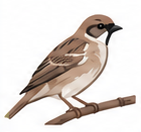
\includegraphics[width=13mm,height=11.5mm,keepaspectratio]{figures/06-foundations/02-learning-theory/tikz/learning-theory-conditional-information/assets/bird.png}};
\node[inner sep=0pt] at (29,41) {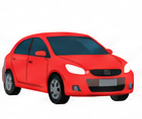
\includegraphics[width=13mm,height=11.5mm,keepaspectratio]{figures/06-foundations/02-learning-theory/tikz/learning-theory-conditional-information/assets/car.png}};
\node[v3 label] at (11,29) {$(1,0)$};\node[v3 label] at (29,29) {$(2,1)$};
\node[v3 title] at (61,52) {同一算法 $A$};
\node[v3 box,draw=FigureGreen,fill=FigureGreen!5!white,minimum width=26mm,minimum height=16mm] (A) at (61,38) {};
% Preserve the original sparse 2--3--1 learner glyph, rather than a generic dense net.
\begin{scope}[shift={(61,38)}]
 \draw[FigureGreen,line width=.8pt] (-7,2)--(0,4)--(7,0) (-7,2)--(0,0)--(7,0) (-7,-2)--(0,0) (-7,-2)--(0,-4)--(7,0);
 \foreach \y in {2,-2}{\draw[FigureBlue!85!FigureStroke,fill=FigureBlue!60!white,line width=.85pt] (-7,\y) circle(1.4);}
 \foreach \y in {4,0,-4}{\draw[FigureYellow!85!FigureStroke,fill=FigureYellow!70!white,line width=.85pt] (0,\y) circle(1.4);}
 \draw[FigureGreen!85!FigureStroke,fill=FigureGreen!75!white,line width=.85pt] (7,0) circle(1.4);
\end{scope}
\node[v3 label,anchor=north] at (61,27) {固定预测 $h(3)=0$\\$h(4)=1$};
\draw[v3 flow,line width=.95pt] (38,38)--(A.west);
\foreach \y/\p/\col in {51/0/FigureBlue,19/1/FigurePurple}{
 \draw[v3 group,draw=\col,fill=\col!4!white,line width=.85pt] (87,{\y-13}) rectangle (162,{\y+14});
 \node[v3 title,text=\col] at (101,{\y+11}) {来源 $\mathcal P_{\p}$};
 \draw[v3 guide,draw=\col] (89,{\y-10}) rectangle (114,{\y+7});
 \node[inner sep=0pt] at (95,{\y+2}) {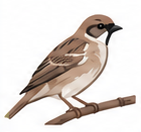
\includegraphics[width=9.5mm,height=8.5mm,keepaspectratio]{figures/06-foundations/02-learning-theory/tikz/learning-theory-conditional-information/assets/bird.png}};
 \node[inner sep=0pt] at (108,{\y+2}) {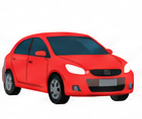
\includegraphics[width=9.5mm,height=8.5mm,keepaspectratio]{figures/06-foundations/02-learning-theory/tikz/learning-theory-conditional-information/assets/car.png}};
 \draw[\col,line width=.6pt] (89,{\y-2.5})--(114,{\y-2.5}) (101.5,{\y-10})--(101.5,{\y+7});
 \node[v3 label] at (95,{\y-6}) {$(1,0)$};\node[v3 label] at (108,{\y-6}) {$(2,1)$};
 \draw[v3 guide] (117,{\y-10})--(117,{\y+11});
 \node[inner sep=0pt] at (137,{\y+8.5}) {
\includegraphics[width=11mm,height=9mm,keepaspectratio]{figures/06-foundations/02-learning-theory/tikz/learning-theory-conditional-information/assets/dog.png}};
 \node[inner sep=0pt] at (153,{\y+8.5}) {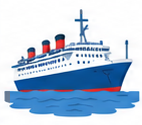
\includegraphics[width=11mm,height=9mm,keepaspectratio]{figures/06-foundations/02-learning-theory/tikz/learning-theory-conditional-information/assets/ship.png}};
 % Scientific table cells retain visual grouping; titles and explanatory notes are unframed.
 \fill[FigureGreenFill,rounded corners=1pt] (118,{\y-2.5}) rectangle (161,{\y+4.5});
 \fill[FigureYellowFill,rounded corners=1pt] (118,{\y-10.5}) rectangle (161,{\y-3.5});
 \draw[FigureGreen,line width=.65pt,rounded corners=1pt] (118,{\y-2.5}) rectangle (161,{\y+4.5});
 \draw[FigureYellow,line width=.65pt,rounded corners=1pt] (118,{\y-10.5}) rectangle (161,{\y-3.5});
 \foreach \xx in {129,145}{\draw[FigureStroke,line width=.45pt] (\xx,{\y-10.5})--(\xx,{\y+4.5});}
 \node[v3 label] at (124,{\y+1}) {真值};\node[v3 label] at (124,{\y-7}) {预测};
 \node[v3 label] at (137,{\y+1}) {$\p$};\node[v3 label] at (153,{\y+1}) {$\p$};
}
\node[v3 label,text=FigureGreen] at (137,44) {$0\;\checkmark$};\node[v3 label,text=FigureRed] at (153,44) {$1\;\times$};
\node[v3 label,text=FigureRed] at (137,12) {$0\;\times$};\node[v3 label,text=FigureGreen] at (153,12) {$1\;\checkmark$};
\draw[v3 flow,line width=.95pt] (A.east)--(80,38)--(80,51)--(87,51);
\draw[v3 flow,line width=.95pt] (80,38)--(80,19)--(87,19);
\node[v3 note] at (125,2) {四个输入等概率，各为 $1/4$};
\end{tikzpicture}
